\begin{frame}{BHD-T0 解析}
  \label{page:BHDT0}
  \tminipageTwo{
    \begin{figure}
      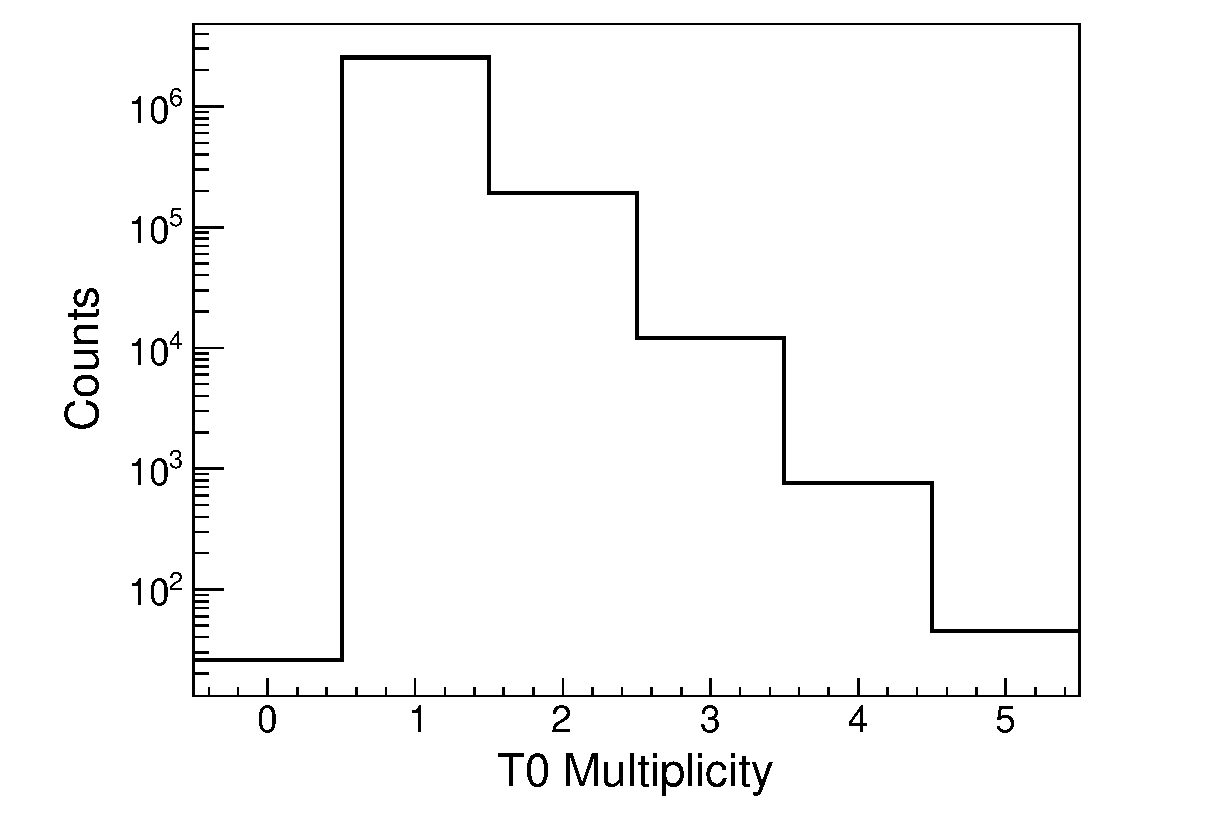
\includegraphics[width=5cm]{../pic/Run78/BL/nT0.eps}
    \end{figure}
  }{
    \begin{figure}
      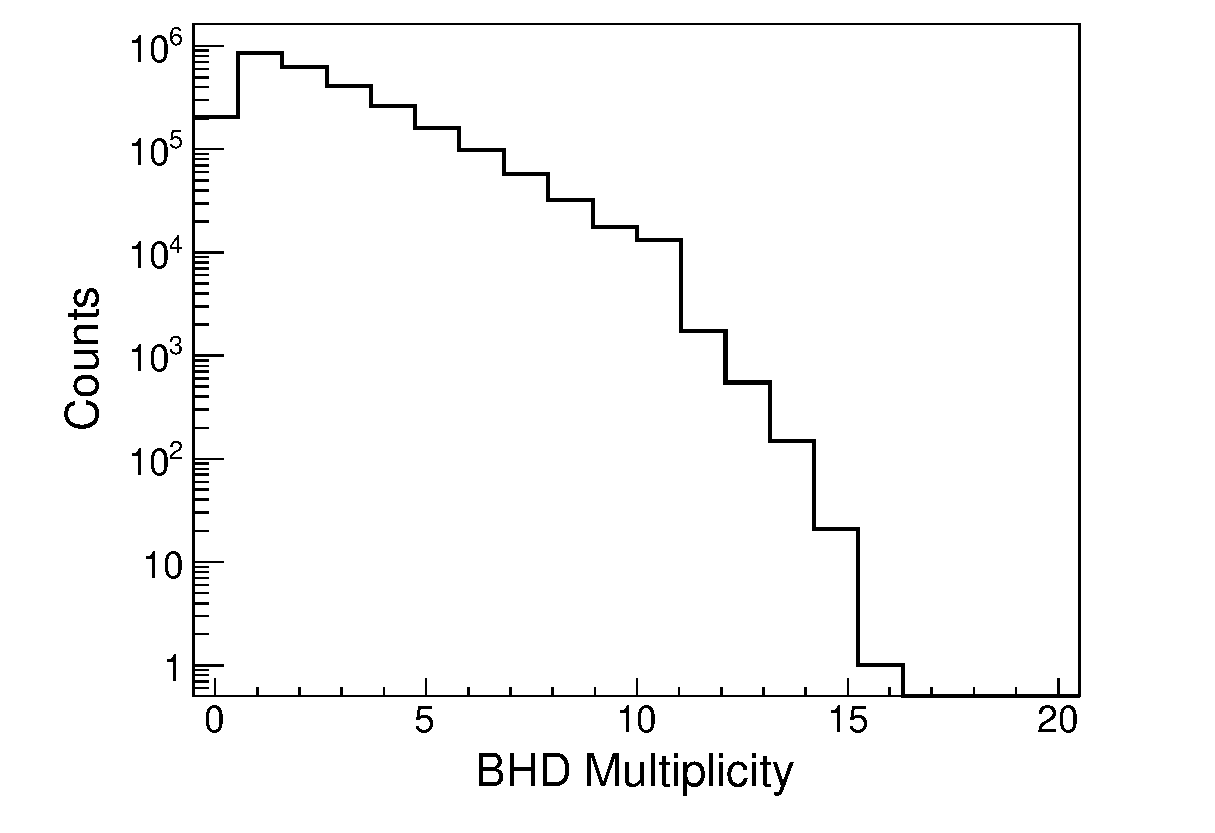
\includegraphics[width=5cm]{../pic/Run78/BL/nBHD.eps}
    \end{figure}
  }

  \tminipageTwo{
    \begin{figure}
      \includegraphics[width=5cm]{../pic/Run78/BL/BHDT0_TOF.eps}
    \end{figure}
  }{
    \hspace{-5mm}
    \scriptsize
    \begin{itemize}
    \item T0が1ヒットのイベントを選ぶ\\
      BHDの1hitはイベントを減らしすぎる\\ので要求しない
    \item BHD-T0 TOFは3$\sigma$で要求(赤領域)。
    \end{itemize}
  }
\end{frame}
